\begin{titreTice}[Généralités sur les fonctions]

\Titre{Tracé de courbe}{0}
\end{titreTice}

\subsection*{Problème}

On souhaite résoudre l'équation $\sqrt{x^2+x+1}=x+2$.
Comme cela parait assez compliqué, on peut conjecturer dans un premier temps les valeurs solutions grâce à la calculatrice.

\subsection*{Mise en ouvre }

\subsubsection*{Tracé des courbes}

\begin{enumerate}
\item On trace la courbe de la fonction $f$ définie sur $\R$ par $f(x)=\sqrt{x^2+x+1}$.
\item On trace la courbe de la fonction $f$ définie sur $\R$ par $g(x)=x+2$.
\end{enumerate}

\begin{minipage}{7.5cm}

\subsection*{Casio}
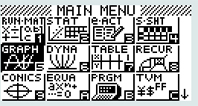
\includegraphics[scale=0.6]{casio0.jpg} 
\vspace{0.3cm}
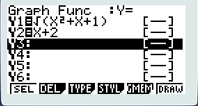
\includegraphics[scale=0.6]{casio1.jpg}

 
Utiliser la touche F6, DRAW pour tracer les 2 courbes.

\end{minipage}\hspace{1cm}
\begin{minipage}{7.5cm}

\subsection*{TI}
Utiliser la touche Y= (haut gauche).

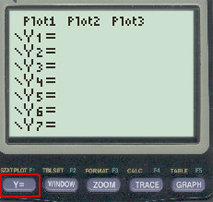
\includegraphics[scale=0.5]{TI0.jpg} 
\vspace{0.3cm}
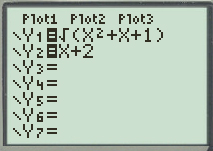
\includegraphics[scale=0.5]{TI1.jpg}
 
Utiliser la touche GRAPH, pour tracer les 2 courbes.
\end{minipage}



\subsubsection*{Lecture}
On lit, sur l'axe des abscisse, l'abscisse des points éventuels d'intersection.
\vspace{0.5cm}

\begin{minipage}{7.5cm}
\section*{Casio}
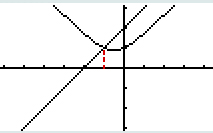
\includegraphics[scale=0.5]{casio2.jpg}
\end{minipage} \hspace{1cm}
\begin{minipage}{7.5cm}
\section*{TI}
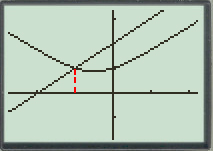
\includegraphics[scale=0.5]{TI2.jpg}
\end{minipage}

\vspace{0.5cm}
\begin{center}
 \fbox{$S=\left\lbrace -1 \right\rbrace$ }
\end{center}


\subsection*{Application}

Une ficelle longue de 20cm est fixée à ses extrémités par deux clous A et B distants de 13 cm.

Est il possible de tendre la ficelle de manière à ce que le triangle ABC soit rectangle en C ?
